\documentclass[11pt]{article}
\usepackage[margin=1in]{geometry}
\usepackage{amsmath,amssymb,amsthm,booktabs,graphicx}
\usepackage[T1]{fontenc}
\usepackage{lmodern,microtype}
\usepackage[colorlinks=true,linkcolor=blue,urlcolor=blue]{hyperref}
\newtheorem{proposition}{Proposition}
\newcommand{\norm}[1]{\left\|#1\right\|}
\newcommand{\R}{\mathbb R}
\newcommand{\C}{\mathbb C}
\title{Learned Transport Corrections: What the Loss Measures,\\
What the Experiments Establish, and a Safeguarded Subspace Formulation}
\author{NPBS project audit and handover note}
\date{12 September 2026}
\begin{document}
\maketitle
\begin{abstract}
This note distinguishes algebraic identities, proved finite-dimensional facts,
numerical observations, and open design questions. The main observation is not
that learning fails for radiative transfer: a trained correction can outperform
four classical correction stages on an average one-step metric while producing
substantially worse Krylov convergence. We document the discrete problem,
classical bases, learned architectures, explicit objectives, historical evidence,
and a new three-seed controlled experiment. A residual-minimizing wrapper has a
proved individual-step safeguard, but its added cost is not justified by a solver
speedup in the present experiment. No production-transport or generalization
theorem is claimed.
\end{abstract}

\section{Scope and provenance}
The audited checkout started at Git revision \texttt{389b95d}. The companion
\path{docs/research/PROJECT_AUDIT_2026_09_12.md} identifies code repairs and
reproduction commands. Historical reports are preserved. An extractor,
\path{scripts/summarize_rte_evidence.py}, checks 360 traces associated with
184 result rows from 15 selected historical CSVs and records source hashes and
locations in \path{docs/research/historical_evidence.tsv}. This is a targeted
audit, not a rerun of every historical experiment.

The original Helmholtz configurations and the RTE experiments are not a
controlled equation-only comparison. For example, the Helmholtz CurveVelA ppw14
PAFNO configuration requests 3,000 velocity fields, 400 epochs, batch 30, a
five-level physics-aware network, Born-metric loss, absorbing padding, and
float64 inference. Most historical RTE trials use a single fixed medium, 12 or
24 angular ordinates, a real-channel gated U-Net, and float32/complex64 arithmetic.
The Helmholtz configuration is source-verified here, not independently retrained.
Its reported success cannot identify the cause of a different experiment's
failure. Both discrete Born identities pass small float64 verification tests.

\section{Discrete transport problem}
Let the spatial domain be the torus $[0,1)^2$, discretized by $N^2$ points with
$h=1/N$. There are $L$ equally spaced directions on $S^1$,
\[
 \theta_l=2\pi l/L,\quad \Omega_l=(\cos\theta_l,\sin\theta_l),\quad w_l=1/L.
\]
The stored field belongs to $\C^{L\times N\times N}$. Spatial differentiation
is pseudo-spectral: the streaming symbol is $i\Omega_l\cdot k$ with
$k=2\pi\,\operatorname{fftfreq}(N,d=h)$ in each coordinate. Define
\begin{equation}\label{eq:A}
 A\psi=\Omega\cdot\nabla_h\psi+\sigma_t\psi-\sigma_s P\psi,
 \qquad A\psi=q,\qquad 0\leq\sigma_s(x)<\sigma_t(x).
\end{equation}
Here $(P\psi)_l=\sum_m w_m p_{lm}\psi_m$. For $|g|<1$, the circular
Poisson kernel $(1-g^2)/(1-2g\cos(\theta_l-\theta_m)+g^2)$ is normalized so
that $\sum_m w_m p_{lm}=1$. At $g=0$, $p_{lm}=1$.
The discrete norm is
\[
 \norm{v}_h^2=\frac{h^2}{L}\sum_{l,i,j}|v_{lij}|^2.
\]
The prefactor cancels in relative residuals but not in definitions of the
operator. This is a periodic $S^1$ prototype, not $S^2$ transport with vacuum,
inflow or reflecting boundaries. There are no upwind sweeps or positivity claims.

\begin{proposition}[Discrete accretivity, exact arithmetic]\label{prop:acc}
For the equally spaced, exactly normalized circular phase matrix above,
let $\alpha=\min_x(\sigma_t-\sigma_s)>0$. Then
\[
 \operatorname{Re}\langle v,Av\rangle_h\geq\alpha\norm{v}_h^2,
 \qquad \norm{A^{-1}}_h\leq\alpha^{-1}.
\]
\end{proposition}
\begin{proof}
The Fourier streaming matrix is skew-Hermitian. The phase matrix $P$ is real
symmetric, nonnegative and doubly stochastic, since its kernel is circulant.
Its spectral norm is at most one: its induced one- and infinity-norms are one,
so its two-norm is at most their geometric mean. At each spatial point the
Hermitian collision matrix $\sigma_t I-\sigma_s P$ is bounded below by
$(\sigma_t-\sigma_s)I$. Summation proves the first assertion. Cauchy--Schwarz
then gives $\norm{Av}_h\geq\alpha\norm{v}_h$, and finite dimensionality gives
invertibility and the second assertion.
\end{proof}
This proposition concerns the ideal discrete matrices, up to roundoff in their
implementation. It neither proves contraction of a chosen splitting nor makes
the matrix normal. Streaming and collision need not commute.

\section{Classical bases and defect2}
Let $\bar\sigma_t$ and $\bar\sigma_s$ be spatial means, and set
\[
 \eta=10^{-6}+\eta_{\rm scale}\max_x
       (|\sigma_t-\bar\sigma_t|+\sigma_s),\qquad
 G=(\Omega\cdot\nabla_h+\bar\sigma_t+\eta)^{-1}.
\]
Writing $V=G^{-1}-A$ gives $I-GV=GA$ by multiplication. This is an identity,
not a learned-convergence theorem. The supported base maps are:
\begin{align*}
 B_{\rm Born}r&=Gr,\\
 B_{\rm DSA}r&=Gr+\mathcal L D^{-1}\mathcal R(r-AGr),\\
 D&=-d\Delta_h+(\bar\sigma_t-\bar\sigma_s),\qquad d=(2\bar\sigma_t)^{-1},\\
 B_{\rm TSA}r&=Gr+T^{-1}(r-AGr),\\
 \widehat T(k)&=\operatorname{diag}_l(i\Omega_l\cdot k+\bar\sigma_t+\eta)
                      -\bar\sigma_s P.
\end{align*}
The scalar moment is $\mathcal Rv=L^{-1}\sum_l v_l$ and $\mathcal L$ repeats
a scalar field over all directions. DSA here is a periodic constant-reference
diffusion augmentation, not a transport-consistent heterogeneous DSA scheme.
In particular $d$ does not incorporate the anisotropic transport cross section.

Full TSA uses all $L$ angular components. TSA-M4 uses nine Fourier modes
$0,\pm1,\ldots,\pm4$ in a closed projected reference inverse. In contrast,
TSA4 means four successive defect stages, not four angular modes. For a fixed
linear unit-relaxation base $B$, define
\[
 C_j(r)=\sum_{s=0}^{j-1}B(I-AB)^s r.
\]
Telescoping gives $I-AC_j=(I-AB)^j$. The two-stage learned map is
\begin{equation}\label{eq:defect}
 z_0=Br,\quad z_1=B(r-Az_0),\qquad
 M_\theta(r)=z_0+\omega z_1+\delta_\theta(z_0,z_1;a).
\end{equation}
Coefficient features are denoted by $a$. With zero output and $\omega=1$, this
is $C_2$. The legacy bias-free gated U-Net is real-linear in residual channels
for fixed coefficients, absent optional residual-dependent heads. Its
coefficient encoder is nonlinear in $a$; real-linearity is not complex-linearity.

The full-angular architecture Fourier-transforms the two stage fields in angle,
retains all modes, uses grouped periodic spatial convolutions, coefficient gates
and mode mixing at every spatial scale, and adds a low-rank mode mixer plus a
residual-energy gate. It is generally nonlinear in the residual. Grouped skip
concatenation was repaired to preserve per-mode channel blocks. Its low-rank
perturbation now has the form
\[
 K(a)=r^{-1}\sum_{j=1}^r a_j(a)u_jv_j^T,
 \quad |a_j|\leq s,\quad \norm{u_j},\norm{v_j}\leq1,
 \quad\norm{K(a)}_2\leq s.
\]
The bound follows from the triangle inequality for rank-one norms. It does not
bound the complete network or imply contraction.

If $Q_4$ is the fixed retained angular basis, corrections of the form
$Q_4 H_\theta Q_4^*$ remain in its range, even with nonlinear coefficient maps
or residual-dependent weights. The existing learned moment R/P class changes
matrices inside this range around a fixed coarse inverse. It is not an
A-aware learned Galerkin space. A genuinely new range requires fine-space
columns outside $Q_4$ and a specified small solve; adding parameters inside
$Q_4$ cannot achieve that.

\section{Losses and the missing implication}
For an input residual $r\ne0$, define
\[
 e_\theta(r)=r-AM_\theta(r),\qquad
 \rho(r)=\frac{\norm{e_\theta(r)}}{\norm r},\qquad
 \rho_B(r)=\frac{\norm{Be_\theta(r)}}{\norm{Br}}.
\]
The physical loss is $\mathbb E\rho^2$; the metric loss is
$\mathbb E\rho_B^2$. Neither equals $\mathbb E\rho$, its square, or the
single-source quantity $\rho(q)$. Rollout ratios may normalize each new defect
by its current input. Correction-teacher and action-teacher discrepancies are,
respectively,
\[
 \frac{\norm{M(r)-C_4(r)}^2}{\norm{C_4(r)}^2},\qquad
 \frac{\norm{A(M(r)-C_4(r))}^2}{\norm r^2}.
\]

\begin{proposition}[Covariance-weighted objective]\label{prop:cov}
For a fixed real-linear map, use Euclidean real-stacked fields and put $E=I-AM$ and
$C=\mathbb E[rr^T/\norm r^2]$. Then
\[
 \mathbb E\rho(r)^2=\operatorname{tr}(ECE^T).
\]
For a bank of $m$ residuals, $\operatorname{rank}C\leq m$. For isotropic
unit-sphere residuals in real dimension $d$, the loss is $\norm E_F^2/d$.
Here $C$ is an uncentered second moment, not a mean-subtracted covariance.
If $\lambda_+(C)$ denotes its smallest positive eigenvalue and $\Pi$ its
range projector, then $\norm{E\Pi}_2^2\leq L_{\rm phys}/\lambda_+(C)$.
\end{proposition}
\begin{proof}
Expand $r^TE^TEr/\norm r^2$ as a trace and take expectations. The finite-bank
covariance is a sum of $m$ rank-one matrices. Rotational symmetry and trace one
give $C=I/d$ for isotropic residuals.
Finally $C\succeq\lambda_+(C)\Pi$ implies
$\operatorname{tr}(ECE^T)\geq\lambda_+(C)\norm{E\Pi}_F^2
\geq\lambda_+(C)\norm{E\Pi}_2^2$.
\end{proof}
The loss alone imposes no constraint on $E$ on $\ker C$; this does not exclude
architecture-induced generalization beyond the bank. The rank statement concerns
the original empirical bank, not a population distribution or adaptive replay.
Small average loss therefore need not control poorly sampled directions,
$\norm E_2$, powers of $E$, or future Krylov spaces. Nonlinear models do not
admit this single fixed $E$ representation. No such implication is assumed.

\section{Evidence and explicit experiment settings}
Historical full12 U-Net training at size 64 and 14,400 updates uses 5,949
residual entries from one mixed medium, width 16, four levels, batch 256 and
physical plus correction-teacher loss. Its sampled loss falls from .293390
to .095186 and sampled one-step ratio from .319635 to .210184. The heldout
source ratio is .111631 versus TSA4's .114459; a later continuation reaches
.107681. Yet its first trace crossing of $10^{-5}$ takes 15 iterations and
.202553 seconds, versus TSA4's 11 and .101581 seconds in the same final record.
The learned method uses 30 base calls versus 44: base-call equality is not
wall-time equality. Its approximately $8\cdot10^{-6}$ tail at 40 iterations
does not meet the configured $10^{-6}$ tolerance. A precision explanation is
plausible but requires a matching higher-precision experiment.

The new laptop experiment uses the same periodic operator with $N=16$, $L=12$,
$g=.65$, $\eta_{\rm scale}=.1$, full TSA and complex64. The mixed medium has
attenuation .35 on $x<.48$ and 16 otherwise, plus
$2\exp[-120(x-.5)^2]$, with albedos .20 and .985. Both networks use three
levels and coefficient width 16; the angular network uses four hidden channels
per angular mode. Legacy and angular parameter counts are 71,872 and 131,499.
Training uses AdamW, learning rate .001 with cosine decay to .00001, weight
decay .0001, clipping norm 1, batch 16 and 300 updates.

Three seeds vary network initialization and source centers, not the medium.
There are eight training, two validation and three test sources per seed,
cycling beam, dipole and isotropic profiles. Six classical residual stages
per source plus 16 random smooth-action probes give normalized banks of
64, 28 and 34 residuals. The train covariance rank is at most 64 in real
dimension $2L N^2=6144$. Checkpoint selection uses validation-source real-stacked
FGMRES at step zero and every 50 updates; test sources do not select weights.
The solver budget is 12 applications and tolerance $10^{-6}$. CPU timings use
one Torch thread, include solver work, and exclude training and coefficient
setup. All extra operator calls of the new wrapper are charged.
Probe fractions differ across splits: 25, 57.1 and 47.1 percent. Validation
has no isotropic source. Within-split method comparisons remain valid, but
cross-split loss gaps alone cannot diagnose generalization error.

\begin{table}[ht]
\centering\small
\begin{tabular}{lrrrrr}
\toprule
Method & Train loss & Val. loss & Test loss & FGMRES res. & Seconds\\
\midrule
TSA2 & .26809 & .15730 & .19370 & $4.07\,10^{-4}$ & .01309\\
TSA4 & .14667 & .08896 & .10171 & $2.76\,10^{-6}$ & .02209\\
Legacy raw & .13446 & .08474 & .08675 & $2.10\,10^{-4}$ & .02849\\
Angular raw & .17425 & .09611 & .12070 & $3.61\,10^{-4}$ & .06105\\
MR legacy & .12507 & .07781 & .07902 & $2.10\,10^{-4}$ & .04283\\
Projected angular & .12192 & .07322 & .07809 & $2.54\,10^{-4}$ & .07796\\
MR classical4 & .07523 & .04295 & .04941 & $2.85\,10^{-6}$ & .03689\\
\bottomrule
\end{tabular}
\caption{Means over three seeds. Losses are mean squared physical residuals on
fixed banks at selected checkpoints. Solver columns average three untouched
test sources per seed. ``Projected angular'' includes the deployed MR wrapper.
This is a fixed-budget comparison, not timing to a common tolerance.}
\end{table}

Legacy raw has lower test-bank loss than TSA4, but approximately 76 times its
FGMRES residual. Angular seed 3 reduces full-bank train loss from .2648 to
.1031 while validation FGMRES worsens from $5.029\,10^{-4}$ to
$6.376\,10^{-4}$; selection retains step zero. A pure physical objective has
not resolved the missing implication in Proposition~\ref{prop:cov}.
The gain is concentrated in later classical-trajectory states: the test
trajectory loss is .162567 for legacy versus .192014 for TSA4, whereas stage-zero
loss is .048726 versus .026128 and random-probe loss .001451 versus .000113.
At equal 24 base calls, legacy's 12 Krylov iterations do outperform six TSA4
iterations ($2.096\,10^{-4}$ versus $8.303\,10^{-4}$), but the neural overhead
still prevents a measured wall-time win. Equal iterations are not equal work.

Thirty-step power searches on $E^TE$ supply witnessed one-step ratios near
.90 for both TSA2 and trained legacy, versus .78 for TSA4. Applying 12
stationary corrections to these respective witnesses retains .183--.187 for
legacy versus .034 for TSA4. These are lower-bound witnesses, not certified
operator norms. The legacy witnesses contain 17.5--19.0 percent angular energy
outside M4 and 23.2--54.6 percent spatial energy outside the probe-solution
cutoff. Because coefficients vary, $A$ can create high frequencies even from a
filtered probe. These observations motivate difficult-residual replay but do
not prove that replay will cure the limitation.

\begin{figure}[p]
\centering
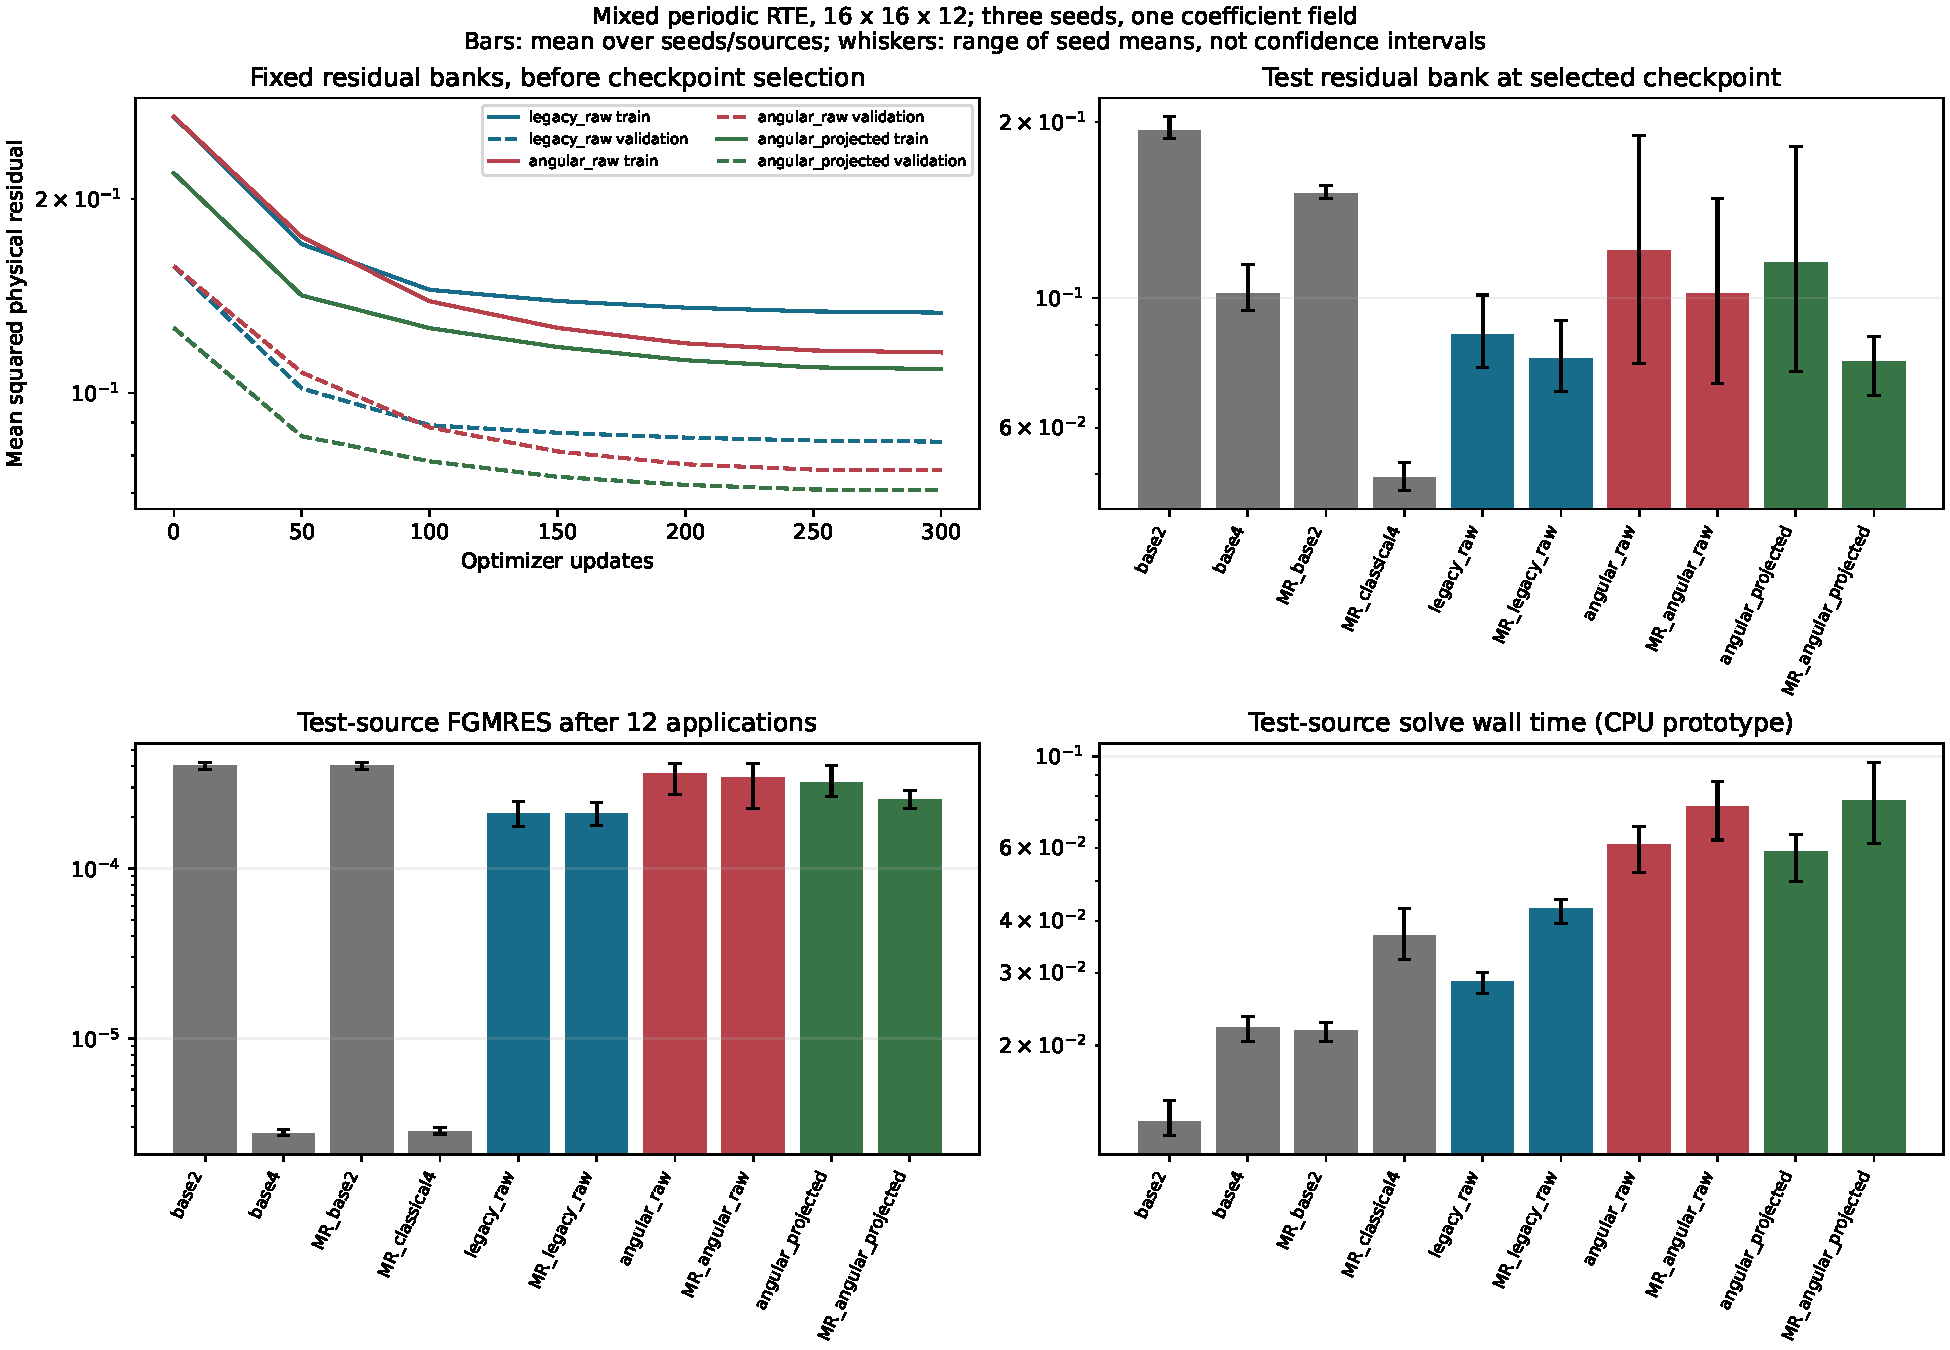
\includegraphics[width=\textwidth]{rte/results/residual_subspace_mixed/comparison.pdf}
\caption{Fixed-bank training curves and selected-checkpoint comparisons.
Whiskers show ranges of seed means, not confidence intervals over independent
media. Full CSVs are stored beside this figure.}
\end{figure}

\section{A safeguarded residual-subspace correction}
Let $b=C_2(r)$ and let $Q$ contain the learned correction and $b$ itself. Normalize
each column by its (detached) action norm with a positive floor, obtaining
$\widetilde Q$. Use real coefficients on complex fields, equivalently real
stacking, and solve
\begin{equation}\label{eq:fit}
 c_\lambda=\arg\min_{c\in\R^k}
 \norm{r-A(b+\widetilde Qc)}^2+\lambda\norm c^2,\quad\lambda=10^{-6}.
\end{equation}
The implementation accumulates the small real Gram system in float64, then
forms the correction in model precision. It explicitly evaluates true residuals
of zero, $b$, the fitted correction, and each $b+q_j$, selecting the least
finite score. This includes the native learned correction $b+\delta$.

\begin{proposition}[Individual-step safeguard]\label{prop:guard}
In exact arithmetic, the fitted correction in \eqref{eq:fit} has residual norm
at most $\norm{r-Ab}$. Selecting a candidate by its true residual gives a norm
no larger than that of any included finite candidate, in particular zero,
the classical correction, and the native learned correction.
\end{proposition}
\begin{proof}
The strictly convex ridge objective has a unique minimizer, even with dependent
or zero columns. Compare its value with the feasible coefficient vector $c=0$
and discard the nonnegative ridge penalty. The candidate-selection statement
is the definition of the finite minimum.
\end{proof}
Finite-precision candidate evaluation protects against a numerically poor fit
to the accuracy of the residual computations. Proposition~\ref{prop:guard}
does not imply a uniform factor below one, Krylov convergence, or domination
of the future classical trajectory. Rejected steps may stagnate.

The forward training loss is
\[
 L_{\rm projected}+0.25L_{\rm native}.
\]
The native term can supply a nonzero derivative at zero learned output; a pure
subspace-fitting loss can have a zero-output stationary point. Differentiation
uses detached column normalization and the selected candidate branch, hence a
surrogate derivative rather than the exact derivative of the displayed forward
objective with positive ridge. For a fixed baseline, the native derivative is
\[
 DL_{\rm native}[v]=-2\mathbb E
 \frac{\operatorname{Re}\langle r-Ab,A\,D\delta[v]\rangle}{\norm r^2}.
\]
It can vanish for an exact baseline, tangent orthogonality or cancellation. Tests
compare against an independent real-stacked least-squares solve, verify
gradients, dependent columns and nonzero zero-output training gradients.
This is a classical residual-minimization construction used to test a learning
interface, not a claim of novelty.

The classical control is given the same two-direction fit with
$b=C_2(r)$ and $q=C_2(r-Ab)$, so it uses four base calls in total. The new
wrapper is not faster than plain TSA4. Its tested improvement is one-step
safeguarding, not competitive neural acceleration.

\section{Concrete next trials and implementation boundaries}
The implemented \texttt{legacy\_replay} arm retains the same architecture and
physical loss, replaces one quarter of each minibatch by four detached
difficult residuals, and refreshes them by 15 power iterations every 50 updates.
It uses only the training medium and current model. Extra probe cost is logged;
matched updates do not imply matched training cost. This is exploratory.
The three-seed run has mean test-bank loss .08754 versus .08675 for raw
legacy, and test-source FGMRES residual $2.188\,10^{-4}$ versus
$2.096\,10^{-4}$. Witnessed one-step ratios decrease to .882--.884, but
12-step stationary ratios remain .184--.187. This small replay intervention
does not establish a solver improvement and is not promoted to a default.

Next distinguish three questions: can the network correct the witnessed slow
directions; can it retain this ability along actual Krylov trajectories; and
is the reduction worth inference cost? Test actual residual/basis replay and
action-teacher loss before increasing capacity indiscriminately. A short
differentiable Krylov objective or a method retaining multiple learned
directions could better match the generated space, but requires its own
classical augmentation controls. ROM-enhanced FGMRES offers a relevant
comparison \cite{peng}; its transport discretization and reduced spaces are
not the network studied here.

The repaired large-ensemble plan separates nested 256/4096-sample datasets at
128,000 updates. The latter uses 2,000 full passes; the former 32,000, with
matched teacher/evaluation update schedules. These runs have not been executed.
Distinct train, validation and test media, fixed-probe heldout losses, strict
cache fingerprints, complete epoch-boundary restart state, and actual-device
metadata are now recorded. Requested unavailable CUDA execution fails rather
than silently falling back. Exact resume was tested on CPU, not CUDA.

Acceptance requires lower time to a common true-residual tolerance on untouched
sources and media, with failure rates, precision, setup and amortized training
cost reported. Unit tests, a small one-step loss, a reduced base-call count,
or a selected checkpoint are individually insufficient. No theorem of learned
uniform contraction or new-subspace superiority is claimed.

\begin{thebibliography}{9}
\bibitem{peng} Z. Peng, \emph{A Flexible GMRES Solver with Reduced Order Model
Enhanced Synthetic Acceleration Preconditioner for Parametric Radiative Transfer
Equation}, arXiv:2410.08735, version 3.
\url{https://arxiv.org/html/2410.08735v3}.
\end{thebibliography}
\end{document}
